%	MODULO PER LA COMUNICAZIONE
% socket
% passaggio ip
% protocollo comunicazione

La comunicazione fra i robot � stata implementata tramite socket tcp. Tale tecnologia ci ha permesso, tramite la conoscenza pregressa degli indirizzi IP di tutti i robot partecipanti, di costruire delle linee di comunicazione punto-punto. Come gi� visto nella sezione introduttiva, il gioco prevede due ruoli: sono proprio i giocatori di ruoli diversi i soli a doversi scambiare messaggi.

ROS permette la definizione di variabili globali al sistema referenziabili a run time nei diversi nodi. Abbiamo scelto di sfruttare questa possibilit� offerta dal sisterma per comunicare ai robot gli indirizzi IP di tutti i partecipanti, incluso il proprio. I primi memorizzati in una lista di stringhe e il secondo in una semplice stringa, queste variabili vengono settate una volta sola (dopo aver eseguito roscore) attraverso le due istruzioni seguenti e recuperate nel metodo \texttt{\_\_init\_\_} del nodo \texttt{RoleManager}.
\begin{center}
	\texttt{setparam /ipList "['100.101.0.10', '100.101.0.11', '100.101.0.11']"}
	\texttt{setparam /myIPAddress "100.101.0.10"}
\end{center}

\subsection{Il Protocollo di Comunicazione}
	Il protocollo di comunicazione � molto semplice. La struttura statica del gioco ci ha permesso di definire un protocollo rigido. I messaggi vengono scambiati solo tra giocatori di ruoli diversi, in particolare tra i Kids e la Witch: questo spiega la scelta di collegamenti punto-punto.
	
	Sono stati previsti tre tipi di messaggio:
	\begin{itemize}
		\item un messaggio in cui la Witch comunica a tutti i Kids il colore da toccare, dando cos� il via al gioco;
		\item un messaggio in cui un Kid comunica alla Witch di aver appena toccato il colore comunicatogli;
		\item un messaggio in cui la Witch comunica a tutti i Kids che il gioco � terminato e chi � il perdente, il quale sar� la prossima Witch.
	\end{itemize}
	Una descrizione grafica del protocollo di comunicazione � presentata in Figura~\ref{fig:communicationprotocol}
	
	% Figura di una contrazione
	\begin{figure}
		\centering
		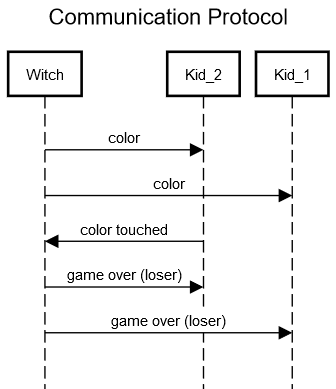
\includegraphics[width=0.7\textwidth]{images/CommunicationProtocol.png}
		\caption{Rappresentazione grafica del protocollo di comunicazione.}
		\label{fig:communicationprotocol}
	\end{figure}